\chapter{Introduction}

Drug (Figure \ref{Background:Drugs}) discovery is an expensive and long-term business. It takes about US\$1.8 billion over 13.5 years to develop a new drug \citep{716}.

\begin{figure}[h]
\centering
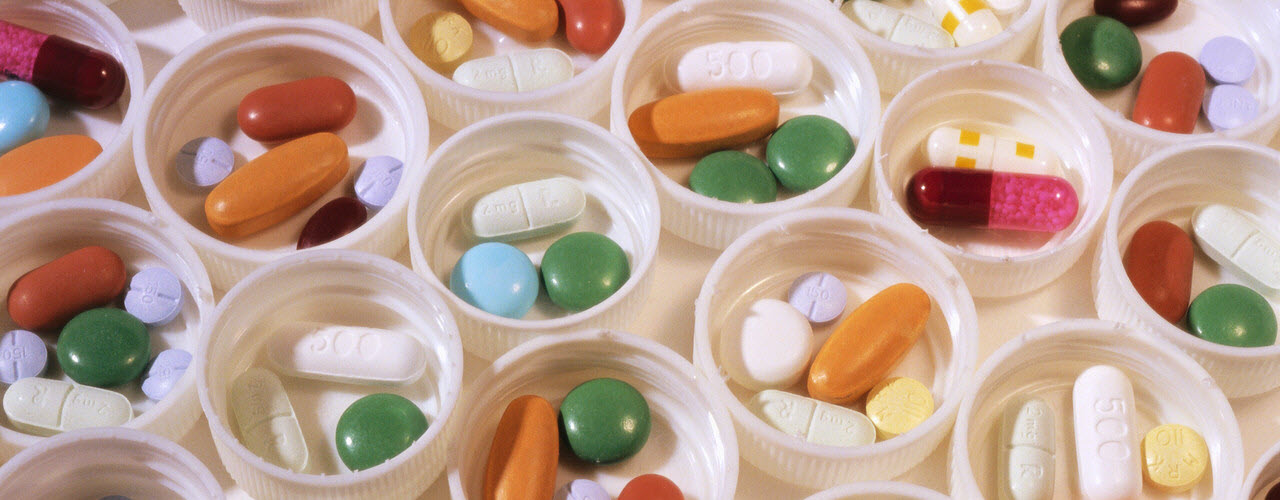
\includegraphics[width=\textwidth]{Background/Drugs.jpg}
\caption{Drugs.}
\label{Background:Drugs}
\end{figure}

\section{Motivation}

Drug discovery via biological and chemical means alone are both cost- and time-inefficient. It highlights the need for cheaper and faster method, and computer-aided drug discovery thus comes into the scene. Over recent decades, researchers have developed countless tools and utilities, and more are constantly emerging. We surveyed those tools and utilities, and summarized the major problems they suffer from. Generally speaking, they
\begin{enumerate}
\item are commercially available, selling at a price that most small enterprises and academic researchers cannot afford,
\item are proprietary and closed source, making it difficult for others to learn inner implementation techniques and locate possible bugs,
\item conform to different standards and adopt different input/output formats, resulting in loss of valuable information during format conversion,
\item require intensive and tedious configurations and lack fruitful documentations, a great obstacle for others to set up the program properly,
\item run very slowly, using old-fashioned, blocking, single-threaded, low-performance programming style,
\item are declared dead immediately upon their initial release due to zero maintenance afterward.
\end{enumerate}
Therefore, we are going to address these shortcomings.

\section{Objective}

We aim to develop a novel and concise computational framework for modern drug discovery. Our framework shall
\begin{enumerate}
\item be free to the general public so that everyone can obtain it,
\item be released under permissive open source licenses so that everyone can study it,
\item be designed in conformance to a uniform and well-accepted standard so that everyone can use it with ease,
\item provide a SaaS (Software as a Service) platform with a HTML5- and CSS3-powered responsive web site so that everyone can play with it,
\item utilize multithreading and GPU acceleration to boost performance so that everyone can really benefit from it,
\item track bugs, absorb user feedback, and release new versions regularly so that everyone can keep using it.
\end{enumerate}

\section{Progress}

Table \ref{Introduction:Progress} roughly estimates the current progress of our projects and case studies. So far, we have developed idock for structure-based protein-ligand docking. We released idock 1.0 in July 2011. Compared with state-of-the-art AutoDock Vina \citep{595}, idock 1.0 obtained a speed up of 6.3x to 10.4x, resulting in a screening performance of 1.3 drug-like ligands per CPU minute. We then released idock 1.1 in December 2011, idock 1.2 in February 2012, idock 1.3 in March 2012, idock 1.4 in April 2012, and idock 1.5 in June 2012, further improving docking speed, adding new functionalities, and fixing bugs. idock 1.5 outperformed AutoDock Vina by 10x. With idock 1.5, we are now conducting massive protein-ligand docking experiments as real-life case studies for our colleagues and collaborators.

Moreover, on one hand, we are building istar as a SaaS platform for idock in order to automate the protein-ligand docking process. On the other hand, we are working on igrow for computational ligand synthesis in order to produce novel potent compounds.

\begin{table}
\centering
\begin{tabular*}
{\linewidth}
{@{\extracolsep{\fill}}lr}
\toprule
\multicolumn{2}{r}{\textbf{Progress}}\\
\midrule
\multicolumn{2}{l}{\textbf{Projects}}\\
idock 1.0: Protein-Ligand Docking \citep{1153} & 100\% \\
idock 1.5: Protein-Ligand Docking (submitted to a journal) & 100\% \\
idock 2.0: GPU Acceleration &  5\% \\
idock 3.0: Ligand Synthesis & 50\% \\
istar: SaaS Platform (submitted to a journal) & 100\% \\
\noalign{\smallskip\smallskip}
\multicolumn{2}{l}{\textbf{Case studies}}\\
Influenza A Virus H1N1 & 90\% \\
Tumors and Carcinomas & 50\% \\
Cancer Stem Cells & 0\% \\
\bottomrule
\end{tabular*}
\caption{Current progress of our projects and case studies.}
\label{Introduction:Progress}
\end{table}

\section{Outline}

Chapter 2 serves as a concise literature survey on computer-aided drug discovery, gives an overview of the pharmaceutical industry and introduces several hot research problems we are currently working on. Chapter 3 presents our tool idock for protein-ligand docking. Chapter 4 presents our SaaS platform istar. Chapter 5 describes our proposal. Chapter 6 introduces three on-going real-life drug discovery case studies. Chapter 7 concludes the thesis proposal. Appendix A lists my publications.

\chapterend
